\documentclass{beamer}

\usepackage[utf8]{inputenc}
\usepackage[russian]{babel}
\usepackage{hyperref}
\usepackage{graphicx}
\usepackage{listings}
\usepackage{cmap}

\usetheme{Warsaw}
\usecolortheme{lily}
\useoutertheme[subsection=false]{smoothbars}
\useinnertheme{circles}
\setbeamertemplate{footline}[page number]{}
\setbeamertemplate{navigation symbols}{}

\title{Архитектура ЭВМ}
\subtitle{Лекция 2. GaLyA}
\author{к.ф.-м.н. Филонов Павел Владимирович \\ filonovpv@gmail.com}
\date{9 сентября 2013 г.}

\institute[МГТУ ГА] 
{
    Московский Государственный Технический Университет \\
    Гражданской Авиации
}
\begin{document}
    \frame{\titlepage}
    \begin{frame}{О чём поговорим сегодня?}
        \begin{enumerate}
            \pause
            \item О некоторых СС 
            \pause
            \item "Вычитать и умножать, малышей не обижать учат в школе, учат в школе, учат в школе"
            \pause
            \item KiD хорош, но GaLyA лучше
            \pause
            \item Поднять флаги!
            \pause
            \item Прыг-скок и условные переходы
            \pause
            \item Никаких {\tt if, for, while}, только {\tt jump}, только hardcore!
        \end{enumerate}
    \end{frame}

    \section{СС}
    \subsection{}
    \begin{frame}{СС бывают разные}
        \begin{block}{Десятичная --- наша любимая}
            No comments
        \end{block}
        \begin{block}{Двоичная --- любимица современных ЭВМ}
        $11001101_2 = 1 \cdot 2^7 + 1 \cdot 2^6 + 0 \cdot 2^5 + 0 \cdot 2^4
            + 1 \cdot 2^3 + 1 \cdot 2^2 + 0 \cdot 2^1 + 1 \cdot 2^0 = 205$ \\
        $75 = 64 + 8 + 2 + 1 = 2^6 + 2^3 + 2^1 + 2^0 = 1001011b$
        \end{block}
        \begin{block}{Восьмеричная --- встречается в кодах прав доступа UNIX}
            $$
                0755 = 0111101101b \hbox{ --- rwxr-xr-x}
            $$
        \end{block}
        \begin{block}{Шестнадцатеричная --- <<Компромисс>> между десятичной и двоичной}
            0x3F = 00111111b = 077 = 63 \\
            A1h = 10100001b = 0241 = 161
        \end{block}
    \end{frame}
    \begin{frame}{Степени двойки}
        \begin{table}
            \begin{tabular}{|r|r|r|r|r|}
            \hline i  & $2^i$ & $2^i$b       & 0$2^i$ & 0x$2^i$ \\
            \hline 0  &  1    & 1b           & 01    & 0x1      \\
            \hline 1  &  2    & 10b          & 02    & 0x2      \\
            \hline 2  &  4    & 100b         & 04    & 0x4      \\
            \hline 3  &  8    & 1000b        & 010   & 0x8      \\
            \hline 4  &  16   & 10000b       & 020   & 0x10     \\
            \hline 5  &  32   & 100000b      & 040   & 0x20     \\
            \hline 6  &  64   & 1000000b     & 0100  & 0x40     \\
            \hline 7  &  128  & 10000000b    & 0200  & 0x80     \\
            \hline 8  &  256  & 100000000b   & 0400  & 0x100    \\
            \hline 9  &  512  & 1000000000b  & 01000 & 0x200    \\
            \hline 10 &  1024 & 10000000000b & 02000 & 0x400    \\
            \hline    
            \end{tabular}
        \end{table}
    \end{frame}
    \begin{frame}{Правило тетрад}
        \begin{columns}
        \column{0.4\linewidth}
        \begin{table}\small
            \begin{tabular}{|r|r|r|}
            \hline  $N_{10}$  & $N_2$   & $N_{16}$ \\
            \hline    0     & 0000b   &   0x0  \\
            \hline    1     & 0001b   &   0x1  \\
            \hline    2     & 0010b   &   0x2  \\
            \hline    3     & 0011b   &   0x3  \\
            \hline    4     & 0100b   &   0x4  \\
            \hline    5     & 0101b   &   0x5  \\
            \hline    6     & 0110b   &   0x6  \\
            \hline    7     & 0111b   &   0x7  \\
            \hline    8     & 1000b   &   0x8  \\
            \hline    9     & 1001b   &   0x9  \\
            \hline    10    & 1010b   &   0xA  \\
            \hline    11    & 1011b   &   0xB  \\
            \hline    12    & 1100b   &   0xC  \\
            \hline    13    & 1101b   &   0xD  \\
            \hline    14    & 1110b   &   0xE  \\
            \hline    15    & 1111b   &   0xF  \\
            \hline
            \end{tabular}
        \end{table}
        \column{0.6\linewidth}
        $$
            0xA5 = \underbrace{1010}_{0xA}\underbrace{0101}_{0x5}b
        $$
        $$
            \underbrace{0110}_{0x6}\underbrace{1101}_{0xD}b = 0x6D 
        $$
        \pause
        \only<2>{
            $$
            0x3C = 
            $$
        }
        \only<3->{
            $$
            0x3C = \underbrace{0011}_{0x3}\underbrace{1100}_{0xC}b
            $$        
        }
        \pause
        \only<4>{
            $$
            01011011b = 
            $$
        }
        \only<5->{
            $$
            \underbrace{0101}_{0x5}\underbrace{1011}_{0xB}b = 0x5B
            $$            
        }
        \end{columns}
    \end{frame}
    \section{Машинная арифметика}
    \subsection{}
    \begin{frame}{Машинная арифметика}
    \begin{columns}
    \column{0.7\linewidth}
    Сначала всё в порядке
    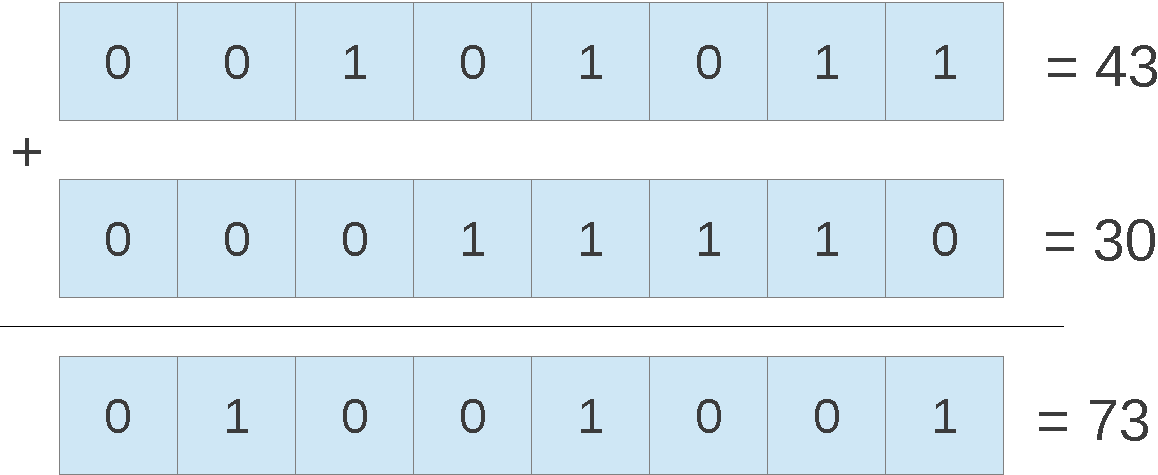
\includegraphics[width=\linewidth]{fig/sum1.pdf} \\
    \pause
    А теперь --- сюрприз!
    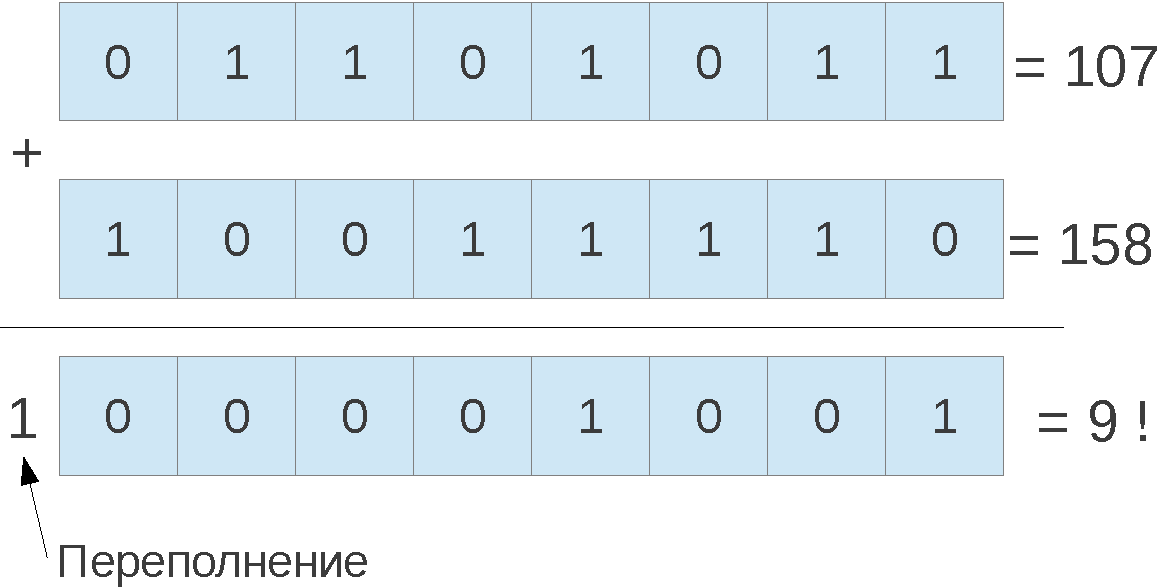
\includegraphics[width=\linewidth]{fig/sum2.pdf}
    \column{0.3\linewidth}
    \pause
        В качестве результата всех операций сложения берётся остаток от деления на $2^n$, где $n$ --- число хранимых двоичных разрядов
        $$
            a + b = (a + b) \mod 2^n
        $$
    \pause
        \begin{eqnarray*}
            107 + 158 &=& \\
            265 \mod 2^8 &=& 9
        \end{eqnarray*}
    \end{columns}
    \end{frame}
    \begin{frame}{Что сложнее --- сложение или вычитание?}
        \begin{block}{А можно ли упростить вычитание?}
        \pause
        $245 - 109 = 245 + 1000 - 1000 - 109 = 245 + 999 + 1 - 109 - 1000 =$ \\
        $ = 245 + (999 - 109) + 1 - 1000 = 245 + 890 + 1 - 1000  = $ \\
        $ = 245 + 891 - 1000 = 1136 - 1000 = 136$
        \end{block}
        \pause
        \begin{block}{Что же мы сделали?}
            Дополнение разрядов $109$ до 9 :$109 \to 999 - 109 = 890$ \\
            Дополнение числа $890$ до 10 : $890 \to 890 + 1 = 891$ \\
            Сложение : $245 + 891 = 1136$ \\
            Простое вычитание : $1136 - 1000 = 136$
        \end{block}
    \end{frame}
    \begin{frame}{Дополнительный код}
        \begin{block}{А как это выглядит в двоичном коде?}
            \begin{itemize}
                \item {\bf Прямой код} --- $00110101b$
                \item Дополнение до 1 (инвертируются все биты) $00110101b \to 11001010b$ --- {\bf обратный код}
                \item Дополнение до 2 ($+1$) $11001010b + 1 = 11001011b$ --- {\bf дополнительный код}
                \item Вычитание заменяется сложением с дополнительным кодом вычитаемого
                \item Переполнение срабатывает как вычитание 1 из старшего разряда (-1000 в предыдущем примере)
            \end{itemize}
        \end{block}
        \pause
        \begin{block}{Пример}
        $81 - 51 = 01010001b - 00110011b = 01010001b + 11001101b = $ \\
        $(1)00011110b = 00011110b = 30$
        \end{block}
    \end{frame}
    \begin{frame}{Представление знаковых чисел}
        \begin{block}{Правила для знаковых чисел}
            \begin{itemize}
                \item Старший бит хранит знак числа (0 - '+', 1 - '-')
                \item Для положительных чисел дополнительный, обратный и прямой коды совпадают
                \item Для отрицательных чисел в дополнительном коде хранятся значащие разряды (все кроме старшего)
            \end{itemize}
        \end{block}
        \begin{block}{Пример}
        $-35 \to 10100011 \to 11011100 \to 11011101$ \\
        $ 101 \to 01100101$
        \end{block}
    \end{frame}
    \begin{frame}{Представление знаковых чисел}
        \begin{table}
        \small
            \begin{tabular}{|p{0.25\linewidth}|r|r|r|} 
            \hline Десятичное представление & Прямой & Обратный & Дополнительный \\
            \hline 127    &  01111111  &  01111111  &  01111111  \\      
            \hline 1      &  00000001  &  00000001  &  00000001  \\     
            \hline 0      &  00000000  &  00000000  &  00000000  \\     
            \hline -1     &  10000001  &  11111110  &  11111111  \\     
            \hline -2     &  10000010  &  11111101  &  11111110  \\     
            \hline -3     &  10000011  &  11111100  &  11111101  \\     
            \hline -4     &  10000100  &  11111011  &  11111100  \\     
            \hline -5     &  10000101  &  11111010  &  11111011  \\     
            \hline -6     &  10000110  &  11111001  &  11111010  \\     
            \hline -7     &  10000111  &  11111000  &  11111001  \\     
            \hline -8     &  10001000  &  11110111  &  11111000  \\     
            \hline -9     &  10001001  &  11110110  &  11110111  \\     
            \hline -10    &  10001010  &  11110101  &  11110110  \\     
            \hline -11    &  10001011  &  11110100  &  11110101  \\     
            \hline -127   &  11111111  &  10000000  &  10000001  \\     
            \hline -128   &  10000000  &  11111111  &  10000000  \\
            \hline
            \end{tabular}
        \end{table}
    \end{frame}
    \begin{frame}{Диапазоны представления целых чисел}
        \begin{table}
            \begin{tabular}{|l|l|l|}
            \hline Размер (байт) & Беззнаковые & Знаковые \\
            \hline   1           &  0..255     & -128..127 \\
            \hline   2           &  0..65535   & -32768..32767 \\
            \hline   3           &  0..16777215 & -8366608..8366607 \\
            \hline   4           &  0..4294967295 & -2147483648..2147483647 \\
            \hline
            \end{tabular}    
        \end{table}
        \begin{block}{Грубое правило для оценки $ 2^{10} \sim 10^3$}
            $2^{16} \sim 10^3 * 2^6 = 64000$ \\
            $2^{24} \sim 10^6 * 2^4 = 16000000$ \\
            $2^{32} \sim 10^9 * 2^2 = 4000000000$ \\
            $2^{64} \sim 10^{18} * 2^4 = 16 *10^{18}$
        \end{block}
    \end{frame}
    \begin{frame}{Разминка (кодирование со знаком)}
        \begin{enumerate}
            \item \alt<2->{$99 - 105=-6=11111010b = 0xFA$}{$99 - 105=$}
            \item<2-> \alt<3->{$45-75=-30=11100010b=0xE2$}{$45-75 = $}
            \item<3-> \alt<4->{$10-111=-101=10011011b = 0x9B$}{$10-111=$}
            \item<4-> \alt<5->{$120+35 = 155 = 10011011и = 0x9B = -101$}{$120 + 35 = $}
            \item<5-> \alt<6->{$-100-79=-179=77 \mod 256 =01001101b=0x4D$}{$-100 - 79 = $}
        \end{enumerate} 
    \end{frame}
    \section{GaLyA}
    \subsection{}
    \begin{frame}{GaLyA (http://cleric.su/galya)}
    \begin{figure}
        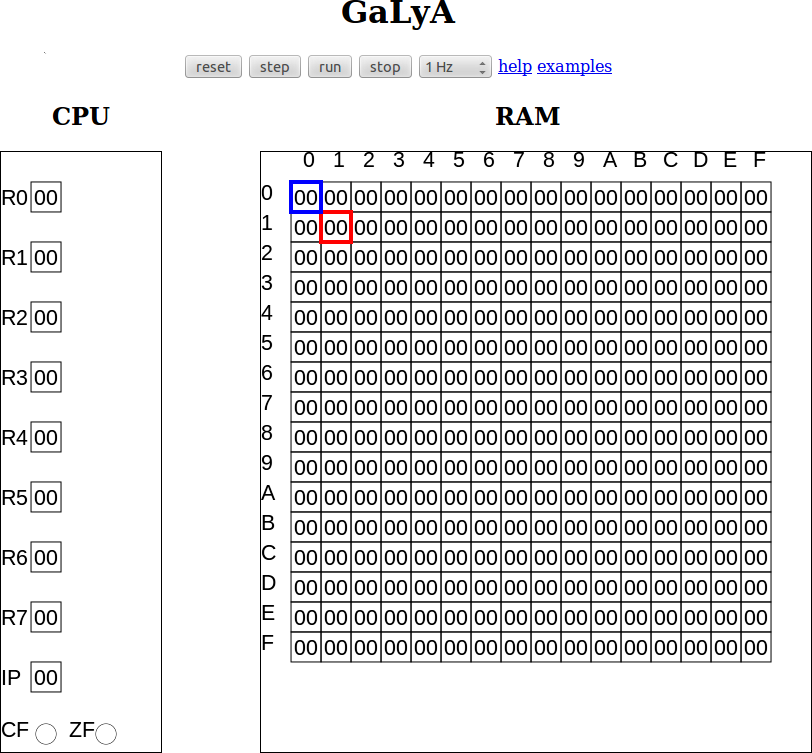
\includegraphics[width=0.7\linewidth]{fig/galya.png}
    \end{figure}
    \end{frame}
    \begin{frame}{Описание архитектуры}
        \begin{enumerate}
            \item Система счисления --- шестнадцатеричная
            \item Разрядность регистров --- 8 бит
            \item Регистры общего назначения --- R0-R7
            \item Счётчик команд --- IP
            \item Объём оперативной памяти --- 256 байт
            \item Тактовая частота (число операций в секунду) --- 1, 2, 5, 10, 100 Гц
            \item Флаги: ZF --- флаг нуля, CF --- флаг переноса
            \item Система команд --- 28 команд
            \item Все арифметические операции производятся только над содержимым регистров!
        \end{enumerate}
    \end{frame}
    \begin{frame}[fragile]
        \frametitle{Пример (арифметические операции)}
        \begin{block}{$0xA6 - 0x23 + 0x45*0x02 = $}
        \begin{verbatim}
 Мнемокод            Машинный код
R0 := 0xA6          0x09 0x00 0xA6
R1 := 0x23          0x09 0x01 0x23
R0 := R0 - R1       0x21 0x00 0x01
R2 := 0x45          0x09 0x02 0x45
R3 := 0x02          0x09 0x03 0x02
R2 := R2 * R3       0x26 0x02 0x03
R0 := R0 + R2       0x20 0x00 0x02
HLT                 0xFF
        \end{verbatim}
        \end{block}
\end{frame}
    \begin{frame}[fragile]
        \frametitle{Пример (адреса памяти)}
        {\bf Метка} --- именованный адрес памяти, используемый в мнемокоде
        \begin{block}{$a - b + c*d = $}
        \begin{verbatim}
 Мнемокод        Адрес   Машинный код
R0 := RAM[a]     0x00:  0x0A 0x00 0x16
R1 := RAM[b]     0x03:  0x0A 0x01 0x17
R0 := R0 - R1    0x06:  0x21 0x00 0x01
R2 := RAM[c]     0x09   0x0A 0x02 0x18
R3 := RAM[d]     0x0C:  0x0A 0x03 0x19
R2 := R2 * R3    0x0F:  0x26 0x02 0x03
R0 := R0 + R2    0x12:  0x20 0x00 0x02
HLT              0x15:  0xFF
a: 0xA6          0x16:  0xA6
b: 0x23          0x17:  0x23
c: 0x45          0x18:  0x45
d: 0x02          0x19:  0x02
        \end{verbatim}
        \end{block}
\end{frame}
    \begin{frame}[fragile]
        \frametitle{Пример (безусловный переход)}
        Команда JMP (jump) может записывать адрес в IP и изменять порядок команд
        \begin{block}{}
        \begin{verbatim}
JMP start        0x00:  0x30 0x06
a: 0xA6          0x02:  0xA6
b: 0x23          0x03:  0x23
c: 0x45          0x04:  0x45
d: 0x02          0x05:  0x02
start:
R0 := RAM[a]     0x06:  0x0A 0x00 0x02
R1 := RAM[b]     0x09:  0x0A 0x01 0x03
R0 := R0 - R1    0x0C:  0x21 0x00 0x01
R2 := RAM[c]     0x0F   0x0A 0x02 0x04
R3 := RAM[d]     0x12:  0x0A 0x03 0x05
R2 := R2 * R3    0x15:  0x26 0x02 0x03
R0 := R0 + R2    0x18:  0x20 0x00 0x02
HLT              0x1B:  0xFF
        \end{verbatim}
        \end{block}
\end{frame}
    \begin{frame}{Флаги и условные переходы}

    {\bf Флаг нуля} (ZF -- zero flag) устанавливается в 1, если результат последней арифметической операции равен нулю. Иначе ZF устанавливается в 0. 

    {\bf Флаг переноса} (CF - carry flag) устанавливается в 1, если в результате последней арифметической операции был перенос старшего разряда. Иначе CF устанавливается в 0.
    \begin{block}{Команда JZ (jump zero) --  прыгнуть, если нуль}
        JZ label \\
        if ZF = 1 then
            IP := label
    \end{block}
    \begin{block}{Команда JNZ (jump nonzero) --  прыгнуть, если не нуль}
    JNZ label \\
    if ZF = 0 then
        IP := label
    \end{block}
    \end{frame}
    \begin{frame}[fragile]
        \frametitle{Пример (алгоритм Евклида)}
        \begin{columns}
            \column{0.3\linewidth}
            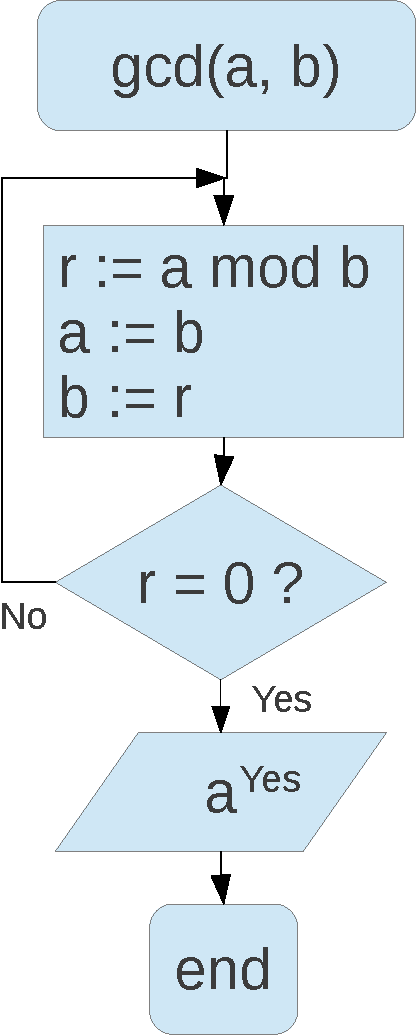
\includegraphics[width=\linewidth]{fig/gcd.pdf}
            \column{0.7\linewidth}
            \begin{verbatim}
JMP start            0x00: 0x30 0x04
a: 0x0F              0x02: 0x0F
b: 0x0A              0x03: 0x0A
start:
  R0 := RAM[a]       0x04: 0x0A 0x00 0x02
  R1 := RAM[b]       0x07: 0x0A 0x01 0x03
loop:
    R2 := R0         0x0A: 0x0C 0x02 0x00
    R2 := R2 mod R1  0x0C: 0x28 0x02 0x01
    R0 := R1         0x10: 0x0C 0x00 0x0C
    R1 := R2         0x13: 0x0C 0x01 0x02
    JNZ loop         0x16: 0x32 0x0A
  HLT                0x18:  0xFF
            \end{verbatim}
        \end{columns}
\end{frame}
    \begin{frame}{Флаги и команда сравнения CMP}

    Команда сравнения CMP RX, RY(compare) вычитает регистр RY из RX, но не сохраняет результат. Зато устанавливает флаги.


    \begin{columns}
        \column{0.75\linewidth}
        Рассмотрим выражение $a - b$ и три возможных случая
        \begin{itemize}\small
            \item[$a > b$:] $a = 20, b = 10$ \\
            $a = 20 = 00010100b, -b = -10 = 11110110b$ \\
            $a + (-b) = (1)00001010b = 00001010b \mod 256$
            \item[$a < b$:] $a = 10, b = 20$ \\
            $a = 10 = 00001010b, -b = -20 = 11101100b$ \\
            $a + (-b) = 00001010b + 11101100b = 11110110b$
            \item[$a = b$:] $a = b = 10$ \\
            $a = 00001010b , -b = -10 = 11110110$ \\
            $a + (-b) = (1)00000000b = 00000000b$
        \end{itemize}
        \column{0.25\linewidth}
            \begin{tabular}{|c|c|c|}
                \hline a,b & ZF & CF  \\
                \hline $a > b$ & 0 & 1 \\
                \hline $a < b$ & 0 & 0 \\
                \hline $a = b$ & 1 & 1 \\
                \hline
            \end{tabular}
    \end{columns}
    \end{frame}
    \begin{frame}{Команды условного перехода}
        \begin{tabular}{|l|l|p{0.4\linewidth}|}
        \hline Мнемоника & Машинный код & Описание \\
        \hline CMP RX, RY & 0x22 0x0X 0x0Y &  RX - RY \\
        \hline JZ XY & 0x31 0xXY & if ZF then IP := 0xXY \\
        \hline JNZ XY & 0x32 0xXY & if not ZF then IP := 0xXY \\
        \hline JE XY & 0x31 0xXY & if ZF then IP := 0xXY \\
        \hline JNE XY & 0x32 0xXY & if not ZF then IP := 0xXY \\
        \hline JL XY & 0x33 0xXY & if not ZF and not ZF then IP := 0xXY \\
        \hline JG XY & 0x34 0xXY & if not ZF and CF then IP := 0xXY \\
        \hline JLE XY & 0x35 0xXY & \alt<2->{if CF = ZF then IP := 0xXY}{} \\
        \hline JGE XY & 0x36 0xXY & \alt<3->{if CF then IP := 0xXY}{} \\
        \hline 
        \end{tabular}
    \end{frame}
    \begin{frame}[fragile]
    \frametitle{Пример --- max(a,b)}
    \begin{verbatim}
if a < b then
    a := b;

Мнемоника          Адрес Машинный код
JMP start          0x00: 0x30 0x04
a:0x34             0x02: 0x34
b:0xA4             0x03: 0xA4
start:
    R0 := RAM[a]   0x04: 0x0A 0x00 0x02
    R1 := RAM[b]   0x07: 0x0A 0x01 0x03
    CMP R0, R1     0x0A: 0x22 0x00 0x01 ; установить ZF,CF
    JGE end        0x0D: 0x36 0x13      ; посмотреть флаги
    MOV R0, R1     0x0F: 0x0C 0x00 0x01
end:
    HLT            0x12: 0xFF
    \end{verbatim}
\end{frame}
    \begin{frame}[fragile]
    \frametitle{Пример --- abs(a - b)}
    \scriptsize
    \begin{verbatim}
if a > b then
    abs := a - b
else
    abs := b - a;

Мнемоника             Адрес Машинный код
JMP start             0x00: 0x30 0x04
a:0x34                0x02: 0x34
b:0xA4                0x03: 0xA4
start:
    R0 := RAM[a]      0x04: 0x0A 0x00 0x02
    R1 := RAM[b]      0x07: 0x0A 0x01 0x03
    CMP R0, R1        0x0A: 0x22 0x00 0x01 ; установить ZF,CF
    JLE else          0x0D: 0x36 0x14      ; посмотреть флаги
then: 
    R0 := R0 - R1     0x0F: 0x21 0x0X 0x01
    JMP end           0x12: 0x30 0x1A      ; безусловный переход
else:
    R1 := R1 - R0     0x14: 0x21 0x01 0x00
    R0 := R1          0x17: 0x0C 0x00 0x01
end:
    HLT               0x1A: 0xFF
    \end{verbatim}
\end{frame}
    \begin{frame}[fragile]
    \frametitle{Пример --- простое число}
    \scriptsize
    \begin{columns}
    \column{0.3\linewidth}
    \begin{verbatim}
    Псевдокод
i := 2;
while i < n do begin
    if n mod i = 0 then 
        return False
    i := i + 1
end;
return True
    \end{verbatim}
    \column{0.7\linewidth}
    \begin{verbatim}
Мнемоника           Адрес Машинный код
JMP start           0x00: 0x30 0x03
n:0x33              0x02: 0x33
start:
  R0 := RAM[a]      0x03: 0x0A 0x00 0x02
  R1 := 2           0x06: 0x09 0x01 0x02
while:
  CMP R1, R0        0x09: 0x22 0x01 0x00  
  JGE wend          0x0C: 0x36 0x21
  if:
    R2 := R0        0x0F: 0x0C 0x02 0x00
    R2 := R2 mod R1 0x12: 0x28 0x02 0x01
    JNZ next        0x15: 0x32 0x1D
  then:
    R0 := 0         0x17: 0x09 0x00 0x00 ; return False
    JMP end         0x1A: 0x30 0x24
next:
  R1 := R1 + 1      0x1D: 0x24 0x01
  JMP while         0x1F: 0x30 0x09
wend:
  R0 := 1           0x21: 0x09 0x00 0x01 ; return True  
end:
    HLT             0x24: 0xFF
    \end{verbatim}
    \end{columns}
\end{frame}
    \begin{frame}[fragile]
    \frametitle{Пример --- числа Фибоначчи}
    \scriptsize
    \begin{columns}
    \column{0.3\linewidth}
    \begin{verbatim}
    Псевдокод
F1 := 0; F2 := 1; F := 0;
for i := 1 to n do begin
    F  := F1 + F2;
    F1 := F2;
    F2 := F;
end;
return F1;
    \end{verbatim}
    \column{0.7\linewidth}
    \begin{verbatim}
Мнемоника             Адрес Машинный код
JMP start             0x00: 0x30 0x03
n:0x10                0x02: 0x10
start:
  R0 := 0x00;   F     0x03: 0x09 0x00 0x00
  R1 := 0x00;   F1    0x06: 0x09 0x01 0x00
  R2 := 0x01;   F2    0x09: 0x09 0x02 0x01
  R4 := RAM[n]; n     0x0C: 0x0A 0x04 0x02
  for:
    R3 := 0x01; i     0x0F: 0x09 0x03 0x01
  cond:   
    CMP R3, R4        0x12: 0x22 0x03 0x04  
    JG  end           0x15: 0x34 0x37
  body:
    R0 := R1          0x17: 0x0C 0x00 0x01
    R0 := R0 + R2     0x2A: 0x20 0x00 0x02
    R1 := R2          0x2D: 0x0C 0x01 0x02
    R2 := R0          0x30: 0x0C 0x02 0x00
    R3 := R3 + 1      0x33: 0x24 0x03
    JMP cond          0x35: 0x30 0x12
end:
  R0 := R1            0x37: 0x0C 0x00 0x01
  HLT                 0x3A: 0xFF
    \end{verbatim}
    \end{columns}
\end{frame}
    \begin{frame}{Краткие итоги}
        \begin{itemize}
            \item Мы знаем как работать с разными СС
            \item Понимаем, в чём особенность машинной арифметики
            \item Можем работать с дополнительными кодами
            \item Придумать свой процессор не очень сложно
            \item Что такое флаги, и как они работают
            \item Что такое команда jump
            \item Как с помощью прыжков имитировать управляющие конструкции (if, for, while)
        \end{itemize}
    \end{frame}

\end{document}